\section{W4: Cryptography}
\textbf{Why cryptography?} \textit{Confidentiality} (only intended parties can read), \textit{Integrity} (only intended parties can write), \textit{Authentication} (only intended parties can read and write by proving their identity), \textit{Non-repudiation} (no party can deny having read or written).

\subsection{Symmetric Encryption}
\textbf{AES:} ciphertext = encrypt(key, plaintext) and plaintext = decrypt(key, ciphertext). AES has different modes of operation.\\
\begin{itemize}
    \item \textbf{Electronic Code Book (ECB):} each block of plaintext is encrypted separately. Simple, parallelisable, but insecure as patterns in plaintext are visible in ciphertext.
    \item \textbf{Cipher Block Chaining (CBC):} each block of plaintext is XORed with previous ciphertext block before encryption. IV can be public, but must be random. If missing ciphertext, it affects at most two blocks, itself and the next one.
    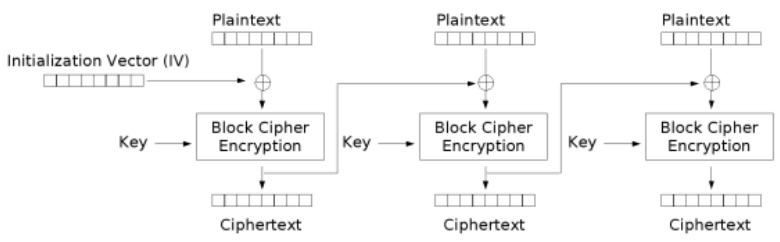
\includegraphics[width=\linewidth]{figs/cbc-encryption.png}
    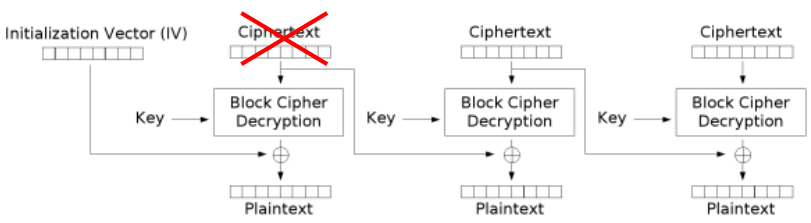
\includegraphics[width=\linewidth]{figs/cbc-decryption.png}
    \item \textbf{Counter (CTR):} each block of plaintext is XORed with a counter value before encryption.
\end{itemize}

\subsection{Asymmetric Encryption}
\textbf{RSA:} ciphertext = encrypt(public key, plaintext) and plaintext = decrypt(private key, ciphertext).\\
\textbf{TLS:} generally uses asymmetric encryption to exchange a symmetric key, then uses symmetric encryption for the rest of the session.\\

\subsection{Digital Signatures}
\textbf{Why digital signatures?} \textit{Authentication}, \textit{Non-repudiation}.\\
\textbf{Why use hash digest before encrypting/signing?} Hash digest usually smaller than message, faster to encrypt/sign. You will send both the message and the encrypted hash digest. The hash digest sent can then be decrypted using public key of author and comparing the hash digest to the hash digest of the long message.\\
